\documentclass[12pt,twoside]{report}

% if you wish to use pgfplot, set this next one to true  
\def\usepgf{true}

% This file contains the packages used in this document

\def\true{true}
% if you wish to use pgfplot, set this next one to tru  
\def\usepgf{false}

\usepackage[utf8]{inputenc}
\usepackage[T1]{fontenc}
\usepackage[french]{babel}
\usepackage[a4paper,width=150mm,top=25mm,bottom=25mm,bindingoffset=6mm]{geometry}

% Some classics
\usepackage[hidelinks]{hyperref}
\usepackage{amsmath}
\usepackage{amssymb}
\usepackage{subcaption}
\usepackage{multicol}
\usepackage{xcolor}
\usepackage{multirow}
\usepackage{tabularx}
\usepackage{array}
\usepackage{graphicx}
\usepackage{caption}
\usepackage{mathdots}
\usepackage{bm}
\usepackage{enumitem}


% Tikz
\usepackage{tikz}
\usetikzlibrary{shapes.geometric}

\ifx\usepgf\true 
  \usepackage{pgfplots} 
  \pgfplotsset{width=10cm,compat=1.9} 
  \usepgfplotslibrary{external} % pour exporter séparément les figures et les importer après dans le doc. Compilation plus rapide
  \tikzexternalize[prefix=tikz/]
  \synctex=1 
  \usetikzlibrary{calc}
\fi 





% Change the style of the chapters title pages
\usepackage[Sonny]{fncychap}

% Table of contents at beginning of chapters
\usepackage{minitoc}

% Facyhdr : defines head and foot of pages
\usepackage{fancyhdr}
  \pagestyle{fancy}
  \renewcommand{\chaptermark}[1]{\markboth{#1}{}}
  \renewcommand{\sectionmark}[1]{\markright{#1}{}}
  \fancyhead{}
  \fancyhead[LE]{Chapter \thechapter \hspace{.1em} - \leftmark}
  \fancyhead[RE]{\thepage}
  \fancyhead[RO]{\thesection \hspace{.1em} - \rightmark}
  \fancyhead[LO]{\thepage}
  \fancyfoot{}
  \renewcommand{\headrulewidth}{0.4pt}
  \renewcommand{\footrulewidth}{0.4pt}

% Bibliography
% \usepackage[numbers,sectionbib]{natbib}
% \usepackage{chapterbib} % To layout bibliography of each chapter


% Glossary 
\usepackage[xindy]{glossaries}
	\let\oldnewacronym\newacronym
	\newcommand*{\provideacronym}[3]{%
	  \ifglsentryexists{#1}{%
	  }{%
	    \oldnewacronym{#1}{#2}{#3}%
	  }%
	}
  \makenoidxglossaries
 % Put all the packages (with options) needed in this tex file
% Real and Imaginary
\newcommand{\Rbb}{\mathbb{R}}
\newcommand{\Cbb}{\mathbb{C}}
\newcommand{\e}{e}
\newcommand{\ci}{i}


% Transpose
\renewcommand{\t}{\mathrm{T}}
\newcommand{\h}{\mathrm{H}}

% Others
\newcommand{\irm}{\mathrm{i} \,}
\newcommand{\jrm}{\mathrm{j} \,}

% Matrices shortcuts
\newcommand{\arr}[2]{\begin{array}{#1} #2 \end{array}}
\newcommand{\cro}[1]{\begin{bmatrix} #1 \end{bmatrix}}
\newcommand{\aco}[1]{\begin{Bmatrix} #1 \end{Bmatrix}}
\newcommand{\bra}[1]{\begin{pmatrix} #1 \end{pmatrix}}
\newcommand{\sys}[1]{\begin{array}{rcl} #1 \end{array}}
\newcommand{\sysbra}[1]{\left \{ \begin{array}{rcl} #1 \end{array} \right.}

% 1st and 2nd
\newcommand{\st}{\textsuperscript{st} }
\newcommand{\nd}{\textsuperscript{nd} }

% FE matrices
\newcommand{\q}{\mathbf{q}}
\newcommand{\M}{\mathbf{M}}
\newcommand{\D}{\mathbf{D}}
\newcommand{\K}{\mathbf{K}}
\newcommand{\F}{\mathbf{F}}
\newcommand{\B}{\mathbf{B}}
\newcommand{\C}{\mathbf{C}}
\renewcommand{\H}{\mathbf{H}}

% N (in the GHM method)
\newcommand{\Ncal}{\mathbf{\mathcal{N}}}

% GHM matrices
\renewcommand{\v}{\mathbf{v}}
\newcommand{\z}{\mathbf{z}}
\newcommand{\Mt}{\mathbf{\tilde{M}}}
\newcommand{\Dt}{\mathbf{\tilde{D}}}
\newcommand{\Kt}{\mathbf{\tilde{K}}}
\newcommand{\Ft}{\mathbf{\tilde{F}}}
\newcommand{\Bt}{\mathbf{\tilde{B}}}
\newcommand{\Ct}{\mathbf{\tilde{C}}}

% State-space
\renewcommand{\u}{\mathbf{u}}
\newcommand{\y}{\mathbf{y}}
\newcommand{\x}{\mathbf{x}}
\newcommand{\E}{\mathbf{E}}
\newcommand{\A}{\mathbf{A}}
\newcommand{\G}{\mathbf{G}}
\renewcommand{\L}{\mathbf{L}}

% G (shear modulus)
\newcommand{\Grm}{\mathrm{G}}

% Snapshots
\newcommand{\R}{\mathbf{R}}
\renewcommand{\S}{\mathbf{S}}
\newcommand{\X}{\mathbf{X}}
\newcommand{\Omegabf}{\mathbf{\Omega}}
\newcommand{\I}{\mathbf{I}}

% Correlation matrix
\newcommand{\Z}{\mathbf{Z}}

% Gramians
\renewcommand{\P}{\mathbf{P}}
\newcommand{\Q}{\mathbf{Q}}

% SVD
\newcommand{\U}{\mathbf{U}}
\newcommand{\Sigmabf}{\mathbf{\Sigma}}
\newcommand{\V}{\mathbf{V}}

% Balanced realization
\newcommand{\T}{\mathbf{T}}
\newcommand{\Phibf}{\mathbf{\Phi}}
\newcommand{\Psibf}{\mathbf{\Psi}}

% Eigendecomposition
\newcommand{\mubf}{\mathbf{a}}
\newcommand{\Lambdabf}{\mathbf{\Lambda}}
\newcommand{\W}{\mathbf{W}}

% Colors used in graphs
\definecolor{gnu_black}{RGB}{0,0,0}
\definecolor{gnu_blue}{RGB}{0,114,189}
\definecolor{gnu_orange}{RGB}{217,83,25}
\definecolor{gnu_violet}{RGB}{126,47,142}
\definecolor{gnu_green}{RGB}{119,172,48}
\definecolor{gnu_purple}{RGB}{162,20,47}
\definecolor{gnu_gold}{RGB}{237,177,32}

% Legend in caption
\newcommand{\LSblackline}{
\begin{tikzpicture}[scale=0.2]
    \protect\filldraw[white] (-2.5,-0.5) -- (2.5,-0.5) -- (2.5,0.5) -- (-2.5,0.5);
    \protect\draw[gnu_black, thick] (-2.5,0) -- (2.5,0);
    % \protect\filldraw[gnu_blue] (-0.5,-0.3) -- (0.5,-0.3) -- (0,0.55);
\end{tikzpicture}
}

\newcommand{\LStriangle}{
\begin{tikzpicture}[scale=0.2]
    \protect\filldraw[white] (-2.5,-0.5) -- (2.5,-0.5) -- (2.5,0.5) -- (-2.5,0.5);
    \protect\draw[gnu_blue, thick] (-2.5,0) -- (2.5,0);
    \protect\filldraw[gnu_blue] (-0.5,-0.3) -- (0.5,-0.3) -- (0,0.55);
\end{tikzpicture}
}

\newcommand{\LSstar}{
\begin{tikzpicture}[scale=0.2]
    \protect\filldraw[white] (-2.5,-0.5) -- (2.5,-0.5) -- (2.5,0.5) -- (-2.5,0.5);
    \protect\draw[gnu_orange, thick, dashed] (-2.5,0) -- (2.5,0);
    % Plus
    \protect\draw[gnu_orange, thick] (-0.5,0) -- (0.5,0);
    \protect\draw[gnu_orange, thick] (0,-0.5) -- (0,0.5);
    % Cross
    \protect\draw[gnu_orange, thick] (-0.5,-0.5) -- (0.5,0.5);
    \protect\draw[gnu_orange, thick] (-0.5,0.5) -- (0.5,-0.5);
\end{tikzpicture}
}

\newcommand{\LSplus}{
\begin{tikzpicture}[scale=0.2]
    \protect\filldraw[white] (-2.5,-0.5) -- (2.5,-0.5) -- (2.5,0.5) -- (-2.5,0.5);
    \protect\draw[gnu_violet, thick, dotted] (-2.5,0) -- (2.5,0);
    % Plus
    \protect\draw[gnu_violet, thick] (-0.5,0) -- (0.5,0);
    \protect\draw[gnu_violet, thick] (0,-0.5) -- (0,0.5);
\end{tikzpicture}
}

\newcommand{\LSrectangle}{
\begin{tikzpicture}[scale=0.2]
    \protect\filldraw[white] (-2.5,-0.5) -- (2.5,-0.5) -- (2.5,0.5) -- (-2.5,0.5);
    \protect\draw[gnu_green, thick, dashdotted] (-2.5,0) -- (2.5,0);
    \protect\filldraw[gnu_green] (-0.5,-0.5) -- (0.5,-0.5) -- (0.5,0.5) -- (-0.5,0.5);
\end{tikzpicture}
}
 % Gather your commands here
\newacronym{pcwe}{PCWE}{Perturbed Convective Wave Equation}
\newacronym{lee}{LEE}{Linearized Euler Equations}
\newacronym{bpf}{BPF}{Blade Passing Frequency }
\newacronym{dns}{DNS}{Direct Numerical Simulation}
\newacronym{rans}{RANS}{Reynolds Averaged Navier Stokes}
\newacronym{urans}{URANS}{Unsteady Reynolds Averaged Navier Stokes}
\newacronym{les}{LES}{Large Eddy Simulation}
\newacronym{des}{DES}{Detached Eddy Simulation}
\newacronym{ddes}{DDES}{Delayed Detached Eddy Simulation}
\newacronym{iddes}{IDDES}{Improved Delayed Detached Eddy Simulation}
\newacronym{lbm}{LBM}{Lattice Boltzmann Method}
\newacronym{cfd}{CFD}{Computational Fluid Dynamics}
\newacronym{fem}{FEM}{Finite Element Method}
\newacronym{fvm}{FVM}{Finite Volume Method}
\newacronym{bem}{BEM}{Boundary Element Method}
\newacronym{dtn}{DtN}{Dirichlet to Neumann}
\newacronym{fpp}{FPP}{Fréquence de Passage de Pales}
\newacronym{hvac}{HVAC}{Heat, Ventilation and Air Conditioning}
\newacronym{sngr}{SNGR}{Stochastic Noise Generation and Radiation}
\newacronym{rpm}{RPM}{Random Particle Mesh}
\newacronym{tdfem}{TD-FEM}{Time Domain Finite Element Method}
\newacronym{lns}{LNS}{Limited Numerical Scales}
\newacronym{ale}{ALE}{Arbitrary Lagrangian Eulerian}

\graphicspath{ {figures/}  {figures/title_page/} } % Add several paths to find pictures

% -------------------------------------------------------------------------
\begin{document}

    % All infos before table of contents
    \begin{titlepage}
    \begin{center}
        
        % UTC header
        \Large
        Université de Technologie de Compiègne\\[.4cm]
        
\includegraphics[height=1.3cm]{utcfull.jpg}
        \vspace{.5cm}
        \hrule
        \vspace{1.2cm}
        
        % Title
        \textbf{A POD-based dynamic substructuring technique for large scale frequency-dependent damped mechanical systems. Application on windshield vibro-acoustic studies}\\[1.2cm]
        
        % Author
        \normalsize
        PhD Thesis submitted by\\
        \large
        \textbf{Alexandre Berthet}\\[.8cm]
        
        % Diploma
        \normalsize
        for the degree of\\
        \large
        \textbf{Doctor of Mechanics}\\[0.8cm]
        
        % Fancy aiming at wowing the reader
        \vfill
        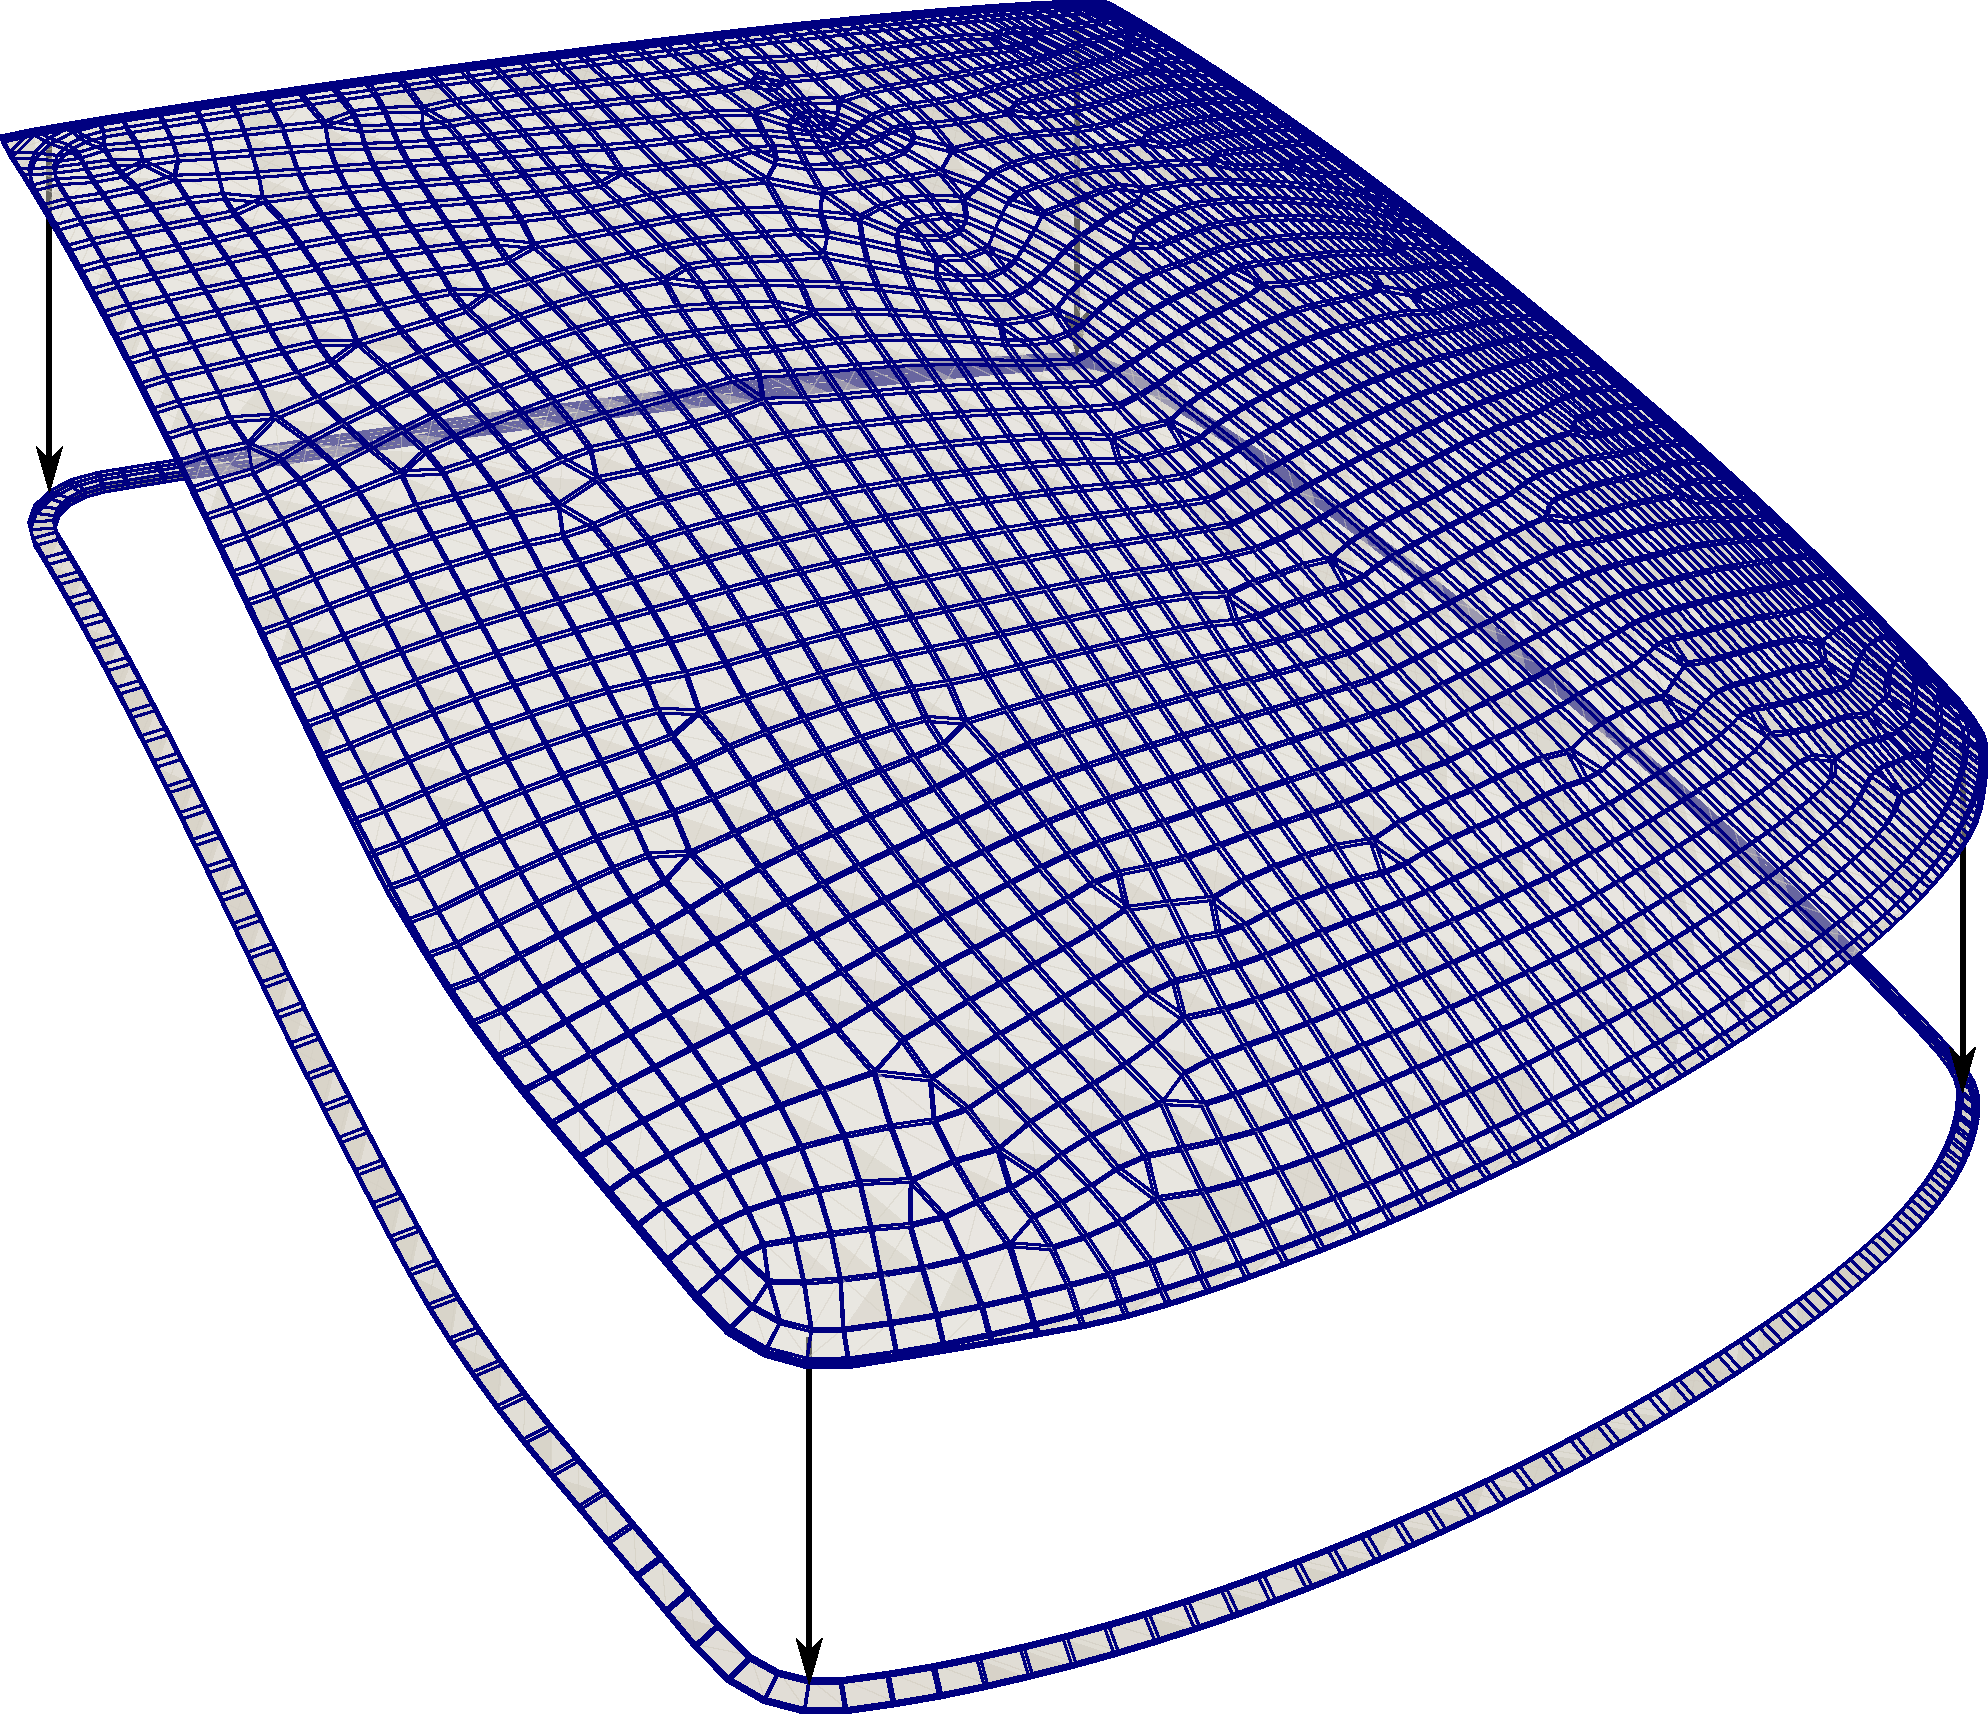
\includegraphics[width=0.7\textwidth]{title_page_picture.pdf}
        \vfill
        
        % Some logos, to respect the obligations of the funders...
		\begin{figure}[b]
    		\centering
    		\def\h{1.2cm} % Change the height of the logos here, once !
    		% 
\includegraphics[height=\h]{logo_fondation_utc.png}
    		% \hfill
    		% 
\includegraphics[height=\h]{logo europe_s_engage_avec_le_feder.jpg}
    		% \hfill
    		% 
\includegraphics[height=\h]{text_FEDER_anglais.png}
    		% \hfill
    		% 
\includegraphics[height=\h]{Logo UE HD.jpg}
    		% \hfill
    		% 
\includegraphics[height=\h]{logo_saint_gobain.png}
		\end{figure}
        
    \end{center}
\end{titlepage}        % Title page
    \chapter*{Abstract}

Lorem ipsum dolor sit amet, consectetur adipisicing elit, sed do eiusmod tempor incididunt ut labore et dolore magna aliqua. Ut enim ad minim veniam, quis nostrud exercitation ullamco laboris nisi ut aliquip ex ea commodo consequat. Duis aute irure dolor in reprehenderit in voluptate velit esse cillum dolore eu fugiat nulla pariatur. Excepteur sint occaecat cupidatat non proident, sunt in culpa qui officia deserunt mollit anim id est laborum.

Lorem ipsum dolor sit amet, consectetur adipisicing elit, sed do eiusmod tempor incididunt ut labore et dolore magna aliqua. Ut enim ad minim veniam, quis nostrud exercitation ullamco laboris nisi ut aliquip ex ea commodo consequat. Duis aute irure dolor in reprehenderit in voluptate velit esse cillum dolore eu fugiat nulla pariatur. Excepteur sint occaecat cupidatat non proident, sunt in culpa qui officia deserunt mollit anim id est laborum.

Lorem ipsum dolor sit amet, consectetur adipisicing elit, sed do eiusmod tempor incididunt ut labore et dolore magna aliqua. Ut enim ad minim veniam, quis nostrud exercitation ullamco laboris nisi ut aliquip ex ea commodo consequat. Duis aute irure dolor in reprehenderit in voluptate velit esse cillum dolore eu fugiat nulla pariatur. Excepteur sint occaecat cupidatat non proident, sunt in culpa qui officia deserunt mollit anim id est laborum.         % Abstract
    \chapter*{Dedication}

\emph{
To mum and dad
}
       % Dedication
    \include{beginning/declarations}     % Declarations
    \chapter*{Acknowledgements}

I would like to thank...
 % Acknowledgements

    % Tables
    \dominitoc
    \clearpage
    \tableofcontents
    \clearpage 
    \listoffigures
    \clearpage 
    \listoftables
    \clearpage 
    \printnoidxglossary % you may comment this if you do not use \gls{entry} for all your acronyms  
    \clearpage 

    % Adds \minitoc and \newpage after calling \chapter{}
    \newcommand{\chapteropts}[1]{\chapter{#1} \minitoc \newpage}

    % for compatibility purposes : comment the following lines and replace them by your personal files
    % Chapters
\chapteropts{Introduction}

\section{Context}

Lorem ipsum dolor sit amet, consectetur adipisicing elit, sed do eiusmod tempor incididunt ut labore et dolore magna aliqua. Ut enim ad minim veniam, quis nostrud exercitation ullamco laboris nisi ut aliquip ex ea commodo consequat. Duis aute irure dolor in reprehenderit in voluptate velit esse cillum dolore eu fugiat nulla pariatur. Excepteur sint occaecat cupidatat non proident, sunt in culpa qui officia deserunt mollit anim id est laborum.

Lorem ipsum dolor sit amet, consectetur adipisicing elit, sed do eiusmod tempor incididunt ut labore et dolore magna aliqua. Ut enim ad minim veniam, quis nostrud exercitation ullamco laboris nisi ut aliquip ex ea commodo consequat. Duis aute irure dolor in reprehenderit in voluptate velit esse cillum dolore eu fugiat nulla pariatur. Excepteur sint occaecat cupidatat non proident, sunt in culpa qui officia deserunt mollit anim id est laborum.

Lorem ipsum dolor sit amet, consectetur adipisicing elit, sed do eiusmod tempor incididunt ut labore et dolore magna aliqua. Ut enim ad minim veniam, quis nostrud exercitation ullamco laboris nisi ut aliquip ex ea commodo consequat. Duis aute irure dolor in reprehenderit in voluptate velit esse cillum dolore eu fugiat nulla pariatur. Excepteur sint occaecat cupidatat non proident, sunt in culpa qui officia deserunt mollit anim id est laborum.

Lorem ipsum dolor sit amet, consectetur adipisicing elit, sed do eiusmod tempor incididunt ut labore et dolore magna aliqua. Ut enim ad minim veniam, quis nostrud exercitation ullamco laboris nisi ut aliquip ex ea commodo consequat. Duis aute irure dolor in reprehenderit in voluptate velit esse cillum dolore eu fugiat nulla pariatur. Excepteur sint occaecat cupidatat non proident, sunt in culpa qui officia deserunt mollit anim id est laborum.

\section{Contents of the manuscript}

Lorem ipsum dolor sit amet, consectetur adipisicing elit, sed do eiusmod tempor incididunt ut labore et dolore magna aliqua. Ut enim ad minim veniam, quis nostrud exercitation ullamco laboris nisi ut aliquip ex ea commodo consequat. Duis aute irure dolor in reprehenderit in voluptate velit esse cillum dolore eu fugiat nulla pariatur. Excepteur sint occaecat cupidatat non proident, sunt in culpa qui officia deserunt mollit anim id est laborum\footnote{This is a footnote.}.

Lorem ipsum dolor sit amet, consectetur adipisicing elit, sed do eiusmod tempor incididunt ut labore et dolore magna aliqua. Ut enim ad minim veniam, quis nostrud exercitation ullamco laboris nisi ut aliquip ex ea commodo consequat. Duis aute irure dolor in reprehenderit in voluptate velit esse cillum dolore eu fugiat nulla pariatur. Excepteur sint occaecat cupidatat non proident, sunt in culpa qui officia deserunt mollit anim id est laborum.

 % Introduction
\chapteropts{State of the art}

\section{Section Title}

Lorem ipsum dolor sit amet, consectetur adipisicing elit, sed do eiusmod tempor incididunt ut labore et dolore magna aliqua. Ut enim ad minim veniam, quis nostrud exercitation ullamco laboris nisi ut aliquip ex ea commodo consequat. Duis aute irure dolor in reprehenderit in voluptate velit esse cillum dolore eu fugiat nulla pariatur. Excepteur sint occaecat cupidatat non proident, sunt in culpa qui officia deserunt mollit anim id est laborum.

Lorem ipsum dolor sit amet, consectetur adipisicing elit, sed do eiusmod tempor incididunt ut labore et dolore magna aliqua. Ut enim ad minim veniam, quis nostrud exercitation ullamco laboris nisi ut aliquip ex ea commodo consequat. Duis aute irure dolor in reprehenderit in voluptate velit esse cillum dolore eu fugiat nulla pariatur. Excepteur sint occaecat cupidatat non proident, sunt in culpa qui officia deserunt mollit anim id est laborum.

Lorem ipsum dolor sit amet, consectetur adipisicing elit, sed do eiusmod tempor incididunt ut labore et dolore magna aliqua. Ut enim ad minim veniam, quis nostrud exercitation ullamco laboris nisi ut aliquip ex ea commodo consequat. Duis aute irure dolor in reprehenderit in voluptate velit esse cillum dolore eu fugiat nulla pariatur. Excepteur sint occaecat cupidatat non proident, sunt in culpa qui officia deserunt mollit anim id est laborum.

Lorem ipsum dolor sit amet, consectetur adipisicing elit, sed do eiusmod tempor incididunt ut labore et dolore magna aliqua. Ut enim ad minim veniam, quis nostrud exercitation ullamco laboris nisi ut aliquip ex ea commodo consequat. Duis aute irure dolor in reprehenderit in voluptate velit esse cillum dolore eu fugiat nulla pariatur. Excepteur sint occaecat cupidatat non proident, sunt in culpa qui officia deserunt mollit anim id est laborum.

Lorem ipsum dolor sit amet, consectetur adipisicing elit, sed do eiusmod tempor incididunt ut labore et dolore magna aliqua. Ut enim ad minim veniam, quis nostrud exercitation ullamco laboris nisi ut aliquip ex ea commodo consequat. Duis aute irure dolor in reprehenderit in voluptate velit esse cillum dolore eu fugiat nulla pariatur. Excepteur sint occaecat cupidatat non proident, sunt in culpa qui officia deserunt mollit anim id est laborum.

\section{Section Title}
Lorem ipsum dolor sit amet, consectetur adipisicing elit, sed do eiusmod tempor incididunt ut labore et dolore magna aliqua. Ut enim ad minim veniam, quis nostrud exercitation ullamco laboris nisi ut aliquip ex ea commodo consequat. Duis aute irure dolor in reprehenderit in voluptate velit esse cillum dolore eu fugiat nulla pariatur see \ref{fig:x cubed graph}. Excepteur sint occaecat cupidatat non proident, sunt in culpa qui officia deserunt mollit anim id est laborum.
\begin{figure}[h]
\centering
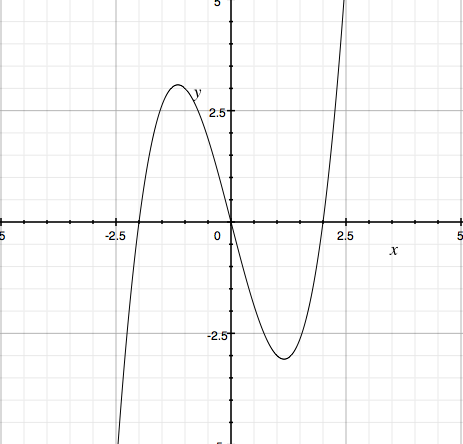
\includegraphics[scale=0.5]{graph_a}
\caption{An example graph}
\label{fig:x cubed graph}
\end{figure}

Lorem ipsum dolor sit amet, consectetur adipisicing elit, sed do eiusmod tempor incididunt ut labore et dolore magna aliqua. Ut enim ad minim veniam, quis nostrud exercitation ullamco laboris nisi ut aliquip ex ea commodo consequat. Duis aute irure dolor in reprehenderit in voluptate velit esse cillum dolore eu fugiat nulla pariatur. Excepteur sint occaecat cupidatat non proident, sunt in culpa qui officia deserunt mollit anim id est laborum.

Lorem ipsum dolor sit amet, consectetur adipisicing elit, sed do eiusmod tempor incididunt ut labore et dolore magna aliqua. Ut enim ad minim veniam, quis nostrud exercitation ullamco laboris nisi ut aliquip ex ea commodo consequat. Duis aute irure dolor in reprehenderit in voluptate velit esse cillum dolore eu fugiat nulla pariatur. Excepteur sint occaecat cupidatat non proident, sunt in culpa qui officia deserunt mollit anim id est laborum.

Lorem ipsum dolor sit amet, consectetur adipisicing elit, sed do eiusmod tempor incididunt ut labore et dolore magna aliqua. Ut enim ad minim veniam, quis nostrud exercitation ullamco laboris nisi ut aliquip ex ea commodo consequat. Duis aute irure dolor in reprehenderit in voluptate velit esse cillum dolore eu fugiat nulla pariatur. Excepteur sint occaecat cupidatat non proident, sunt in culpa qui officia deserunt mollit anim id est laborum.

Lorem ipsum dolor sit amet, consectetur adipisicing elit, sed do eiusmod tempor incididunt ut labore et dolore magna aliqua. Ut enim ad minim veniam, quis nostrud exercitation ullamco laboris nisi ut aliquip ex ea commodo consequat. Duis aute irure dolor in reprehenderit in voluptate velit esse cillum dolore eu fugiat nulla pariatur. Excepteur sint occaecat cupidatat non proident, sunt in culpa qui officia deserunt mollit anim id est laborum.

Lorem ipsum dolor sit amet, consectetur adipisicing elit, sed do eiusmod tempor incididunt ut labore et dolore magna aliqua. Ut enim ad minim veniam, quis nostrud exercitation ullamco laboris nisi ut aliquip ex ea commodo consequat. Duis aute irure dolor in reprehenderit in voluptate velit esse cillum dolore eu fugiat nulla pariatur. Excepteur sint occaecat cupidatat non proident, sunt in culpa qui officia deserunt mollit anim id est laborum.

Lorem ipsum dolor sit amet, consectetur adipisicing elit, sed do eiusmod tempor incididunt ut labore et dolore magna aliqua. Ut enim ad minim veniam, quis nostrud exercitation ullamco laboris nisi ut aliquip ex ea commodo consequat. Duis aute irure dolor in reprehenderit in voluptate velit esse cillum dolore eu fugiat nulla pariatur. Excepteur sint occaecat cupidatat non proident, sunt in culpa qui officia deserunt mollit anim id est laborum.

Lorem ipsum dolor sit amet, consectetur adipisicing elit, sed do eiusmod tempor incididunt ut labore et dolore magna aliqua. Ut enim ad minim veniam, quis nostrud exercitation ullamco laboris nisi ut aliquip ex ea commodo consequat. Duis aute irure dolor in reprehenderit in voluptate velit esse cillum dolore eu fugiat nulla pariatur. Excepteur sint occaecat cupidatat non proident, sunt in culpa qui officia deserunt mollit anim id est laborum.

Lorem ipsum dolor sit amet, consectetur adipisicing elit, sed do eiusmod tempor incididunt ut labore et dolore magna aliqua. Ut enim ad minim veniam, quis nostrud exercitation ullamco laboris nisi ut aliquip ex ea commodo consequat. Duis aute irure dolor in reprehenderit in voluptate velit esse cillum dolore eu fugiat nulla pariatur. Excepteur sint occaecat cupidatat non proident, sunt in culpa qui officia deserunt mollit anim id est laborum.

Lorem ipsum dolor sit amet, consectetur adipisicing elit, sed do eiusmod tempor incididunt ut labore et dolore magna aliqua. Ut enim ad minim veniam, quis nostrud exercitation ullamco laboris nisi ut aliquip ex ea commodo consequat. Duis aute irure dolor in reprehenderit in voluptate velit esse cillum dolore eu fugiat nulla pariatur. Excepteur sint occaecat cupidatat non proident, sunt in culpa qui officia deserunt mollit anim id est laborum.

Lorem ipsum dolor sit amet, consectetur adipisicing elit, sed do eiusmod tempor incididunt ut labore et dolore magna aliqua. Ut enim ad minim veniam, quis nostrud exercitation ullamco laboris nisi ut aliquip ex ea commodo consequat. Duis aute irure dolor in reprehenderit in voluptate velit esse cillum dolore eu fugiat nulla pariatur. Excepteur sint occaecat cupidatat non proident, sunt in culpa qui officia deserunt mollit anim id est laborum.

Lorem ipsum dolor sit amet, consectetur adipisicing elit, sed do eiusmod tempor incididunt ut labore et dolore magna aliqua. Ut enim ad minim veniam, quis nostrud exercitation ullamco laboris nisi ut aliquip ex ea commodo consequat. Duis aute irure dolor in reprehenderit in voluptate velit esse cillum dolore eu fugiat nulla pariatur. Excepteur sint occaecat cupidatat non proident, sunt in culpa qui officia deserunt mollit anim id est laborum.

Lorem ipsum dolor sit amet, consectetur adipisicing elit, sed do eiusmod tempor incididunt ut labore et dolore magna aliqua. Ut enim ad minim veniam, quis nostrud exercitation ullamco laboris nisi ut aliquip ex ea commodo consequat. Duis aute irure dolor in reprehenderit in voluptate velit esse cillum dolore eu fugiat nulla pariatur. Excepteur sint occaecat cupidatat non proident, sunt in culpa qui officia deserunt mollit anim id est laborum.

\section{Section Title}
Lorem ipsum dolor sit amet, consectetur adipisicing elit, sed do eiusmod tempor incididunt ut labore et dolore magna aliqua. Ut enim ad minim veniam, quis nostrud exercitation ullamco laboris nisi ut aliquip ex ea commodo consequat. Duis aute irure dolor in reprehenderit in voluptate velit esse cillum dolore eu fugiat nulla pariatur. Excepteur sint occaecat cupidatat non proident, sunt in culpa qui officia deserunt mollit anim id est laborum.

Lorem ipsum dolor sit amet, consectetur adipisicing elit, sed do eiusmod tempor incididunt ut labore et dolore magna aliqua. Ut enim ad minim veniam, quis nostrud exercitation ullamco laboris nisi ut aliquip ex ea commodo consequat. Duis aute irure dolor in reprehenderit in voluptate velit esse cillum dolore eu fugiat nulla pariatur. Excepteur sint occaecat cupidatat non proident, sunt in culpa qui officia deserunt mollit anim id est laborum.

Lorem ipsum dolor sit amet, consectetur adipisicing elit, sed do eiusmod tempor incididunt ut labore et dolore magna aliqua. Ut enim ad minim veniam, quis nostrud exercitation ullamco laboris nisi ut aliquip ex ea commodo consequat. Duis aute irure dolor in reprehenderit in voluptate velit esse cillum dolore eu fugiat nulla pariatur. Excepteur sint occaecat cupidatat non proident, sunt in culpa qui officia deserunt mollit anim id est laborum.

Lorem ipsum dolor sit amet, consectetur adipisicing elit, sed do eiusmod tempor incididunt ut labore et dolore magna aliqua. Ut enim ad minim veniam, quis nostrud exercitation ullamco laboris nisi ut aliquip ex ea commodo consequat. Duis aute irure dolor in reprehenderit in voluptate velit esse cillum dolore eu fugiat nulla pariatur. Excepteur sint occaecat cupidatat non proident, sunt in culpa qui officia deserunt mollit anim id est laborum.

Lorem ipsum dolor sit amet, consectetur adipisicing elit, sed do eiusmod tempor incididunt ut labore et dolore magna aliqua. Ut enim ad minim veniam, quis nostrud exercitation ullamco laboris nisi ut aliquip ex ea commodo consequat. Duis aute irure dolor in reprehenderit in voluptate velit esse cillum dolore eu fugiat nulla pariatur. Excepteur sint occaecat cupidatat non proident, sunt in culpa qui officia deserunt mollit anim id est laborum.

\subsection{SubSection Title}
Lorem ipsum dolor sit amet, consectetur adipisicing elit, sed do eiusmod tempor incididunt ut labore et dolore magna aliqua. Ut enim ad minim veniam, quis nostrud exercitation ullamco laboris nisi ut aliquip ex ea commodo consequat. Duis aute irure dolor in reprehenderit in voluptate velit esse cillum dolore eu fugiat nulla pariatur. Excepteur sint occaecat cupidatat non proident, sunt in culpa qui officia deserunt mollit anim id est laborum.

\subsection{SubSection Title}
Lorem ipsum dolor sit amet, consectetur adipisicing elit, sed do eiusmod tempor incididunt ut labore et dolore magna aliqua. Ut enim ad minim veniam, quis nostrud exercitation ullamco laboris nisi ut aliquip ex ea commodo consequat. Duis aute irure dolor in reprehenderit in voluptate velit esse cillum dolore eu fugiat nulla pariatur. Excepteur sint occaecat cupidatat non proident, sunt in culpa qui officia deserunt mollit anim id est laborum.
 % Etat de l'art
\chapteropts{Another one bites the dust}

    \section{Section Title}
        Lorem ipsum dolor sit amet, consectetur adipisicing elit, sed do eiusmod tempor incididunt ut labore et dolore magna aliqua. Ut enim ad minim veniam, quis nostrud exercitation ullamco laboris nisi ut aliquip ex ea commodo consequat. Duis aute irure dolor in reprehenderit in voluptate velit esse cillum dolore eu fugiat nulla pariatur. Excepteur sint occaecat cupidatat non proident, sunt in culpa qui officia deserunt mollit anim id est laborum.

        \begin{figure}
            \centering
            \begin{subfigure}[b]{0.3\textwidth}
                \centering
                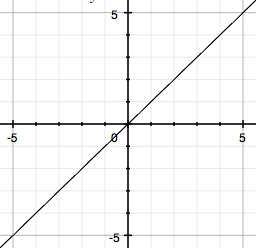
\includegraphics[width=\textwidth]{graph1}
                \caption{$y=x$}
                \label{fig:y equals x}
            \end{subfigure}
            \hfill
            \begin{subfigure}[b]{0.3\textwidth}
                \centering
                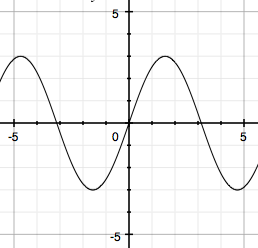
\includegraphics[width=\textwidth]{graph2}
                \caption{$y=3sinx$}
                \label{fig:three sin x}
            \end{subfigure}
            \hfill
            \begin{subfigure}[b]{0.3\textwidth}
                \centering
                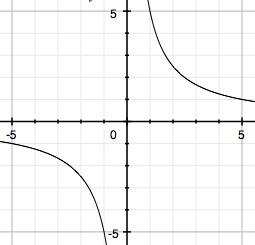
\includegraphics[width=\textwidth]{graph3}
                \caption{$y=5/x$}
                \label{fig:five over x}
            \end{subfigure}
            \caption{Three simple graphs}
            \label{fig:three graphs}
        \end{figure}


        \ifx\usepgf\true 

            \begin{figure}[ht!]
                \centering
                \begin{tikzpicture} [spy using outlines={circle, magnification=3, size=2cm, connect spies}]
                    \begin{axis}
                        [
                            xlabel={un axe quelconque},
                            ylabel={un truc tout aussi quelconque},
                            xmin=100, xmax=3500,
                            ymin=35, ymax=75,
                            legend pos= north east,
                            ymajorgrids=true,
                            xmajorgrids=true,
                            grid style=dashed, 
                            no markers,
                            every axis plot/.append style={ultra thick},
                            width=0.8\textwidth
                        ] 
                        \addplot+ [style=dotted, color=black] table {curves/example/curve1};
                        \addlegendentry{Courbe};
                    \end{axis}
                \end{tikzpicture}
                \caption{Pgfplot rules. End of discussion.}
                \label{fig:pgfplotExample}
            \end{figure}
        \fi 
        
        This curves shows results and has been obtained with the \gls{fem}. 

        
        Lorem ipsum dolor sit amet, consectetur adipisicing elit, sed do eiusmod tempor incididunt ut labore et dolore magna aliqua. Ut enim ad minim veniam, quis nostrud exercitation ullamco laboris nisi ut aliquip ex ea commodo consequat. Duis aute irure dolor in reprehenderit in voluptate velit esse cillum dolore eu fugiat nulla pariatur. Excepteur sint occaecat cupidatat non proident, sunt in culpa qui officia deserunt mollit anim id est laborum.

        Lorem ipsum dolor sit amet, consectetur adipisicing elit, sed do eiusmod tempor incididunt ut labore et dolore magna aliqua. Ut enim ad minim veniam, quis nostrud exercitation ullamco laboris nisi ut aliquip ex ea commodo consequat. Duis aute irure dolor in reprehenderit in voluptate velit esse cillum dolore eu fugiat nulla pariatur. Excepteur sint occaecat cupidatat non proident, sunt in culpa qui officia deserunt mollit anim id est laborum.
        see \ref{fig:five over x}

        Lorem ipsum dolor sit amet, consectetur adipisicing elit, sed do eiusmod tempor incididunt ut labore et dolore magna aliqua. Ut enim ad minim veniam, quis nostrud exercitation ullamco laboris nisi ut aliquip ex ea commodo consequat. Duis aute irure dolor in reprehenderit in voluptate velit esse cillum dolore eu fugiat nulla pariatur. Excepteur sint occaecat cupidatat non proident, sunt in culpa qui officia deserunt mollit anim id est laborum.

        \subsection{SubSection Title}
        Lorem ipsum dolor sit amet, consectetur adipisicing elit, sed do eiusmod tempor incididunt ut labore et dolore magna aliqua. Ut enim ad minim veniam, quis nostrud exercitation ullamco laboris nisi ut aliquip ex ea commodo consequat. Duis aute irure dolor in reprehenderit in voluptate velit esse cillum dolore eu fugiat nulla pariatur. Excepteur sint occaecat cupidatat non proident, sunt in culpa qui officia deserunt mollit anim id est laborum.
 % 
\chapteropts{We might find new titles}

\section{Section Title}
Lorem ipsum dolor sit amet, consectetur adipisicing elit, sed do eiusmod tempor incididunt ut labore et dolore magna aliqua. Ut enim ad minim veniam, quis nostrud exercitation ullamco laboris nisi ut aliquip ex ea commodo consequat. Duis aute irure dolor in reprehenderit in voluptate velit esse cillum dolore eu fugiat nulla pariatur. Excepteur sint occaecat cupidatat non proident, sunt in culpa qui officia deserunt mollit anim id est laborum.

\begin{table}[ht]
\centering
\begin{tabular}{l | l | l}
A & B & C \\
\hline
1 & 2 & 3 \\
4 & 5 & 6
\end{tabular}
\caption{very basic table}
\label{tab:abc}
\end{table}

Lorem ipsum dolor sit amet, consectetur adipisicing elit, sed do eiusmod tempor incididunt ut labore et dolore magna aliqua. Ut enim ad minim veniam, quis nostrud exercitation ullamco laboris nisi ut aliquip ex ea commodo consequat. Duis aute irure dolor in reprehenderit in voluptate velit esse cillum dolore eu fugiat nulla pariatur. Excepteur sint occaecat cupidatat non proident, sunt in culpa qui officia deserunt mollit anim id est laborum.

Lorem ipsum dolor sit amet, consectetur adipisicing elit, sed do eiusmod tempor incididunt ut labore et dolore magna aliqua. Ut enim ad minim veniam, quis nostrud exercitation ullamco laboris nisi ut aliquip ex ea commodo consequat. Duis aute irure dolor in reprehenderit in voluptate velit esse cillum dolore eu fugiat nulla pariatur. Excepteur sint occaecat cupidatat non proident, sunt in culpa qui officia deserunt mollit anim id est laborum.

Lorem ipsum dolor sit amet, consectetur adipisicing elit, sed do eiusmod tempor incididunt ut labore et dolore magna aliqua. Ut enim ad minim veniam, quis nostrud exercitation ullamco laboris nisi ut aliquip ex ea commodo consequat. Duis aute irure dolor in reprehenderit in voluptate velit esse cillum dolore eu fugiat nulla pariatur. Excepteur sint occaecat cupidatat non proident, sunt in culpa qui officia deserunt mollit anim id est laborum.

Lorem ipsum dolor sit amet, consectetur adipisicing elit, sed do eiusmod tempor incididunt ut labore et dolore magna aliqua. Ut enim ad minim veniam, quis nostrud exercitation ullamco laboris nisi ut aliquip ex ea commodo consequat. Duis aute irure dolor in reprehenderit in voluptate velit esse cillum dolore eu fugiat nulla pariatur. Excepteur sint occaecat cupidatat non proident, sunt in culpa qui officia deserunt mollit anim id est laborum.

\section{Section Title}
Lorem ipsum dolor sit amet, consectetur adipisicing elit, sed do eiusmod tempor incididunt ut labore et dolore magna aliqua. Ut enim ad minim veniam, quis nostrud exercitation ullamco laboris nisi ut aliquip ex ea commodo consequat. Duis aute irure dolor in reprehenderit in voluptate velit esse cillum dolore eu fugiat nulla pariatur. Excepteur sint occaecat cupidatat non proident, sunt in culpa qui officia deserunt mollit anim id est laborum.

Lorem ipsum dolor sit amet, consectetur adipisicing elit, sed do eiusmod tempor incididunt ut labore et dolore magna aliqua. Ut enim ad minim veniam, quis nostrud exercitation ullamco laboris nisi ut aliquip ex ea commodo consequat. Duis aute irure dolor in reprehenderit in voluptate velit esse cillum dolore eu fugiat nulla pariatur. Excepteur sint occaecat cupidatat non proident, sunt in culpa qui officia deserunt mollit anim id est laborum.

Lorem ipsum dolor sit amet, consectetur adipisicing elit, sed do eiusmod tempor incididunt ut labore et dolore magna aliqua. Ut enim ad minim veniam, quis nostrud exercitation ullamco laboris nisi ut aliquip ex ea commodo consequat. Duis aute irure dolor in reprehenderit in voluptate velit esse cillum dolore eu fugiat nulla pariatur. Excepteur sint occaecat cupidatat non proident, sunt in culpa qui officia deserunt mollit anim id est laborum.

\section{Section Title}
Lorem ipsum dolor sit amet, consectetur adipisicing elit, sed do eiusmod tempor incididunt ut labore et dolore magna aliqua. Ut enim ad minim veniam, quis nostrud exercitation ullamco laboris nisi ut aliquip ex ea commodo consequat. Duis aute irure dolor in reprehenderit in voluptate velit esse cillum dolore eu fugiat nulla pariatur. Excepteur sint occaecat cupidatat non proident, sunt in culpa qui officia deserunt mollit anim id est laborum.

\begin{table}[h]
    \begin{subtable}[h]{0.45\textwidth}
        \centering
        \begin{tabular}{l | l | l}
        Day & Max Temp & Min Temp \\
        \hline \hline
        Mon & 20 & 13\\
        Tue & 22 & 14\\
        Wed & 23 & 12\\
        Thurs & 25 & 13\\
        Fri & 18 & 7\\
        Sat & 15 & 13\\
        Sun & 20 & 13
        \end{tabular}
        \caption{First Week}
        \label{tab:week1}
    \end{subtable}
    \hfill
    \begin{subtable}[h]{0.45\textwidth}
        \centering
        \begin{tabular}{l | l | l}
        Day & Max Temp & Min Temp \\
        \hline \hline
        Mon & 17 & 11\\
        Tue & 16 & 10\\
        Wed & 14 & 8\\
        Thurs & 12 & 5\\
        Fri & 15 & 7\\
        Sat & 16 & 12\\
        Sun & 15 & 9
        \end{tabular}
        \caption{Second Week}
        \label{tab:week2}
    \end{subtable}
    \caption{Max and min temps recorded in the first two weeks of July}
    \label{tab:temps}
\end{table}

Lorem ipsum dolor sit amet, consectetur adipisicing elit, sed do eiusmod tempor incididunt ut labore et dolore magna aliqua. Ut enim ad minim veniam, quis nostrud exercitation ullamco laboris nisi ut aliquip ex ea commodo consequat. Duis aute irure dolor in reprehenderit in voluptate velit esse cillum dolore eu fugiat nulla pariatur. Excepteur sint occaecat cupidatat non proident, sunt in culpa qui officia deserunt mollit anim id est laborum.

Lorem ipsum dolor sit amet, consectetur adipisicing elit, sed do eiusmod tempor incididunt ut labore et dolore magna aliqua. Ut enim ad minim veniam, quis nostrud exercitation ullamco laboris nisi ut aliquip ex ea commodo consequat. Duis aute irure dolor in reprehenderit in voluptate velit esse cillum dolore eu fugiat nulla pariatur. Excepteur sint occaecat cupidatat non proident, sunt in culpa qui officia deserunt mollit anim id est laborum.

Lorem ipsum dolor sit amet, consectetur adipisicing elit, sed do eiusmod tempor incididunt ut labore et dolore magna aliqua. Ut enim ad minim veniam, quis nostrud exercitation ullamco laboris nisi ut aliquip ex ea commodo consequat. Duis aute irure dolor in reprehenderit in voluptate velit esse cillum dolore eu fugiat nulla pariatur. Excepteur sint occaecat cupidatat non proident, sunt in culpa qui officia deserunt mollit anim id est laborum.

Lorem ipsum dolor sit amet, consectetur adipisicing elit, sed do eiusmod tempor incididunt ut labore et dolore magna aliqua. Ut enim ad minim veniam, quis nostrud exercitation ullamco laboris nisi ut aliquip ex ea commodo consequat. Duis aute irure dolor in reprehenderit in voluptate velit esse cillum dolore eu fugiat nulla pariatur. Excepteur sint occaecat cupidatat non proident, sunt in culpa qui officia deserunt mollit anim id est laborum.

Lorem ipsum dolor sit amet, consectetur adipisicing elit, sed do eiusmod tempor incididunt ut labore et dolore magna aliqua. Ut enim ad minim veniam, quis nostrud exercitation ullamco laboris nisi ut aliquip ex ea commodo consequat. Duis aute irure dolor in reprehenderit in voluptate velit esse cillum dolore eu fugiat nulla pariatur. Excepteur sint occaecat cupidatat non proident, sunt in culpa qui officia deserunt mollit anim id est laborum.

Lorem ipsum dolor sit amet, consectetur adipisicing elit, sed do eiusmod tempor incididunt ut labore et dolore magna aliqua. Ut enim ad minim veniam, quis nostrud exercitation ullamco laboris nisi ut aliquip ex ea commodo consequat. Duis aute irure dolor in reprehenderit in voluptate velit esse cillum dolore eu fugiat nulla pariatur. Excepteur sint occaecat cupidatat non proident, sunt in culpa qui officia deserunt mollit anim id est laborum.

Lorem ipsum dolor sit amet, consectetur adipisicing elit, sed do eiusmod tempor incididunt ut labore et dolore magna aliqua. Ut enim ad minim veniam, quis nostrud exercitation ullamco laboris nisi ut aliquip ex ea commodo consequat. Duis aute irure dolor in reprehenderit in voluptate velit esse cillum dolore eu fugiat nulla pariatur. Excepteur sint occaecat cupidatat non proident, sunt in culpa qui officia deserunt mollit anim id est laborum.

Lorem ipsum dolor sit amet, consectetur adipisicing elit, sed do eiusmod tempor incididunt ut labore et dolore magna aliqua. Ut enim ad minim veniam, quis nostrud exercitation ullamco laboris nisi ut aliquip ex ea commodo consequat. Duis aute irure dolor in reprehenderit in voluptate velit esse cillum dolore eu fugiat nulla pariatur. Excepteur sint occaecat cupidatat non proident, sunt in culpa qui officia deserunt mollit anim id est laborum.

Lorem ipsum dolor sit amet, consectetur adipisicing elit, sed do eiusmod tempor incididunt ut labore et dolore magna aliqua. Ut enim ad minim veniam, quis nostrud exercitation ullamco laboris nisi ut aliquip ex ea commodo consequat. Duis aute irure dolor in reprehenderit in voluptate velit esse cillum dolore eu fugiat nulla pariatur. Excepteur sint occaecat cupidatat non proident, sunt in culpa qui officia deserunt mollit anim id est laborum.
 % 
\chapteropts{It is a chance that is the last one}

Lorem ipsum dolor sit amet, consectetur adipisicing elit, sed do eiusmod tempor incididunt ut labore et dolore magna aliqua. Ut enim ad minim veniam, quis nostrud exercitation ullamco laboris nisi ut aliquip ex ea commodo consequat. Duis aute irure dolor in reprehenderit in voluptate velit esse cillum dolore eu fugiat nulla pariatur. Excepteur sint occaecat cupidatat non proident, sunt in culpa qui officia deserunt mollit anim id est laborum.

Lorem ipsum dolor sit amet, consectetur adipisicing elit, sed do eiusmod tempor incididunt ut labore et dolore magna aliqua. Ut enim ad minim veniam, quis nostrud exercitation ullamco laboris nisi ut aliquip ex ea commodo consequat. Duis aute irure dolor in reprehenderit in voluptate velit esse cillum dolore eu fugiat nulla pariatur. Excepteur sint occaecat cupidatat non proident, sunt in culpa qui officia deserunt mollit anim id est laborum \cite{latexcompanion}.

Lorem ipsum dolor sit amet, consectetur adipisicing elit, sed do eiusmod tempor incididunt ut labore et dolore magna aliqua. Ut enim ad minim veniam, quis nostrud exercitation ullamco laboris nisi ut aliquip ex ea commodo consequat. Duis aute irure dolor in reprehenderit in voluptate velit esse cillum dolore eu fugiat nulla pariatur. Excepteur sint occaecat cupidatat non proident, sunt in culpa qui officia deserunt mollit anim id est laborum \cite{knuthwebsite}.

Lorem ipsum dolor sit amet, consectetur adipisicing elit, sed do eiusmod tempor incididunt ut labore et dolore magna aliqua. Ut enim ad minim veniam, quis nostrud exercitation ullamco laboris nisi ut aliquip ex ea commodo consequat. Duis aute irure dolor in reprehenderit in voluptate velit esse cillum dolore eu fugiat nulla pariatur. Excepteur sint occaecat cupidatat non proident, sunt in culpa qui officia deserunt mollit anim id est laborum \cite{einstein}.
 % 
\chapteropts{Conclusion}

Lorem ipsum dolor sit amet, consectetur adipisicing elit, sed do eiusmod tempor incididunt ut labore et dolore magna aliqua. Ut enim ad minim veniam, quis nostrud exercitation ullamco laboris nisi ut aliquip ex ea commodo consequat. Duis aute irure dolor in reprehenderit in voluptate velit esse cillum dolore eu fugiat nulla pariatur. Excepteur sint occaecat cupidatat non proident, sunt in culpa qui officia deserunt mollit anim id est laborum.

Lorem ipsum dolor sit amet, consectetur adipisicing elit, sed do eiusmod tempor incididunt ut labore et dolore magna aliqua. Ut enim ad minim veniam, quis nostrud exercitation ullamco laboris nisi ut aliquip ex ea commodo consequat. Duis aute irure dolor in reprehenderit in voluptate velit esse cillum dolore eu fugiat nulla pariatur. Excepteur sint occaecat cupidatat non proident, sunt in culpa qui officia deserunt mollit anim id est laborum \cite{latexcompanion}.

Lorem ipsum dolor sit amet, consectetur adipisicing elit, sed do eiusmod tempor incididunt ut labore et dolore magna aliqua. Ut enim ad minim veniam, quis nostrud exercitation ullamco laboris nisi ut aliquip ex ea commodo consequat. Duis aute irure dolor in reprehenderit in voluptate velit esse cillum dolore eu fugiat nulla pariatur. Excepteur sint occaecat cupidatat non proident, sunt in culpa qui officia deserunt mollit anim id est laborum \cite{knuthwebsite}.

Lorem ipsum dolor sit amet, consectetur adipisicing elit, sed do eiusmod tempor incididunt ut labore et dolore magna aliqua. Ut enim ad minim veniam, quis nostrud exercitation ullamco laboris nisi ut aliquip ex ea commodo consequat. Duis aute irure dolor in reprehenderit in voluptate velit esse cillum dolore eu fugiat nulla pariatur. Excepteur sint occaecat cupidatat non proident, sunt in culpa qui officia deserunt mollit anim id est laborum \cite{einstein}.
 % Conclusion


    \clearpage 
    \appendix 
    % Appendices
\appendix
    \chapter{This is the Appendicite}

Text goes here...

    \chapter{Dude, a second one ?}

Text goes here... Again.

    \clearpage 
    \bibliographystyle{plain}
    \bibliography{refs/refs_example.bib}
    
    % %!TEX root = ../main.tex

\input{parameters/myCommands.tex}
\chapter{Intro - contexte - état de l'art}
    % \include{chapters/soa/introduction/introduction}
    \include{chapters/soa/etat_de_lart/etat_de_lart}
    % \include{chapters/soa/problematique/problematique}
    % \include{chapters/soa/approche/approche}
    % \include{chapters/soa/conclusion/conclusion-francaise}



\chapter{Chaînages dans des domaines fixes}
    \label{section:chapDiaphragme}
     \input{chapters/singleDiaphragm/intro.tex}
    \section{Théorie - description de la méthode utilisée}
        \input{chapters/singleDiaphragm/tout}
    \section{Application : simple diaphragme}
        \input{chapters/singleDiaphragm/aero}
    \section{Comparaison de formulations}
        \input{chapters/singleDiaphragm/comparaisonDesFormulations}
    %%%%%% \section{Étude du mapping}
    %%%%%%     \input{chapters/singleDiaphragm/mapping}
    \section{Conclusions}
        \input{chapters/singleDiaphragm/conclusion}

\chapter{Chaînages avec formulations poreuses}
    \label{section:chapPoreux}
    \input{chapters/dAcd/intro.tex}
    \section{Théorie, formulations faibles}
        % %%%%%%%%%%\subsection{Formulation poreuse}
            \input{chapters/dAcd/theorieIntro}
        \subsection{Formulation poreuse 1}
            \input{chapters/dAcd/poreuxCaro}
        \subsection{Formulation poreuse 2}
            \input{chapters/dAcd/poreuxSourcetronquee}
    \section{Application : profil aérodynamique en conduit}
        \subsection{Description du système}
            \input{chapters/dAcd/dacdDef}
        \subsection{Résultats aérodynamiques}
            \input{chapters/dAcd/aero}
            \clearpage 
        \subsection{Résultats acoustiques}
            \input{chapters/dAcd/acoustique}
    \section{Conclusions}
        \input{chapters/dAcd/conclusion}



\chapter{Résolution acoustique dans un domaine tournant 2D}
    \label{section:chap2D}
    \section{Article }
    \section{Compléments à l'article}
        \subsection{détails d'implémentation}
        Projection, matrice des fonctions de base, matrices élémentaires 
        \subsection{calcul d'erreur tc1 avec beaucoup de nLimit différents}
        \subsection{méga système avec C > 2}
        \subsection{solution analytique 1 qui marche mais pas de ouf }
        \subsection{refaire la démo de Kaltenbacher 2016 pour établir l'équation d'onde ur psi en ALE}
        \subsection{Système global}
            % \input{chapters/2d/systemGlobal}
        \subsection{Solution analytique avec la méthode d'Emmanuel}


\chapter{Résolution acoustique dans un domaine tournant 3D}
    \label{section:chap3D}
    \section{Article }
    \section{Compléments à l'article}
        \subsection{comparaison temporel - fréquentiel cas NZE}
        \subsection{Terme source PCWE}
        \subsection{Brouillon}
            \input{chapters/brouillon}




    

    % \clearpage 
    % \appendix 
    % 
    
\chapter{FEM classique }
    \label{section:appendixFEM}
    \begin{itemize}
        \item des calculs d'erreur ? 
        \item \gls{dtn} 
        \item puissance à partir de la \gls{dtn}
    \end{itemize}
    \section{Condition limite Dirichlet to Neumann}
        \input{chapters/appendix/dtn.tex}

% \chapter{Terme source synthétique}
%     tableau des définitions des termes 

\chapter{Étude des conditions de non réflexion des ondes OpenFOAM}
    \label{section:appendixBCCheck}
    \input{chapters/bCCheck/bCCheck.tex}

\chapter{Calcul direct du bruit rayonné par une paire de diaphragmes}
    \label{section:appendixDD}



    % \clearpage 
    % \bibliographystyle{plain}
    % \bibliography{refs/refs.bib}


\end{document}
